\documentclass[10pt]{beamer}
\usetheme{Copenhagen}
\usepackage{amsmath,amsthm,amssymb,amsfonts,mymath}
% \openup 5pt
\author{Blake Farman}
\title{Scaling Laws and Fractals\\
  Section 7.1\\
  Scaling\\
  G.I. Barenblatt\\
}
\institute{
  Department of Mathematics and Statistics\\
  University of Vermont\\
  Burlington, Vermont 05405\\[1ex]
  \texttt{bfarman@cems.uvm.edu}
}
\date{May 03, 2011}

\begin{document}

\theoremstyle{definition}
\newtheorem{defn}{Definition}[section]

\begin{frame}[plain]
  \titlepage
\end{frame}

\begin{frame}{Overview}
  We will introducte the concept of fractal curves and take a look at why their study is of any interest.
  To this end, we will take a look at a couple of examples of fractal curves.
\end{frame}

\begin{frame}{Some History}
  \begin{itemize}
    \item
      Around the 1960's the English physicist L.F. Richardson was commissioned to determine the length of the coast of Britain.
    \item
      Richardson set out using line segments of constant length $\eta$ with vertices along the coastline to approximate the length, $L_{\eta}$.
    \item
      He assumed that by letting $\eta$ tend to zero he could recover $L_{\eta}$ in the limit.
    \end{itemize}
    \begin{center}
      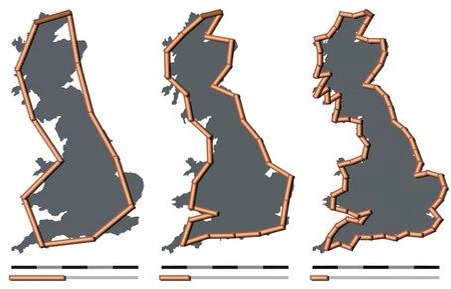
\includegraphics[scale=0.4]{./brit.jpg}\\
      \cite{Wiki}
    \end{center}
\end{frame}

\begin{frame}{Something went awry...}
  Instead of recovering the length of the coastline, Richardson found that the length diverges to infinity as $\eta$ tends to zero.
  Barenblatt assures us that the growth of $L_{\eta}$ follows the scaling law
  \begin{equation}
    \label{1}
    L_{\eta} = \lambda \eta^{1-D},
  \end{equation}
  where $\lambda > 0$ and $1 < D < 2$ are constants.  
\end{frame}

\begin{frame}{}
  \begin{itemize}
  \item
    When different sections of the coastline were approximated, it was seen that the scaling law in \eqref{1} remained valid with the same value of $D$, but a smaller value of $\lambda$.
  \item
    When the coastline of Australia was approximated in a similar way, the scaling law in \eqref{1} was again valid, but this time both $D$ and $\lambda$ changed.
  \item
    The constant $D$ is a dimensionless parameter, however the dimension of $\lambda$ is, oddly enough, a non-integer fractional power of length.
  \end{itemize}
\end{frame}

\begin{frame}{A Simple Example}
  We first consider regular n-gons of length $\eta$ inscribed in a circle of diameter $d$.
  \begin{center}
    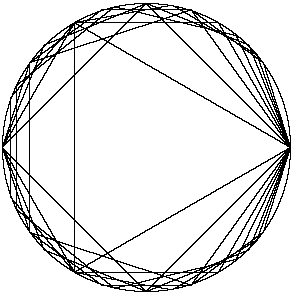
\includegraphics[scale=0.5]{./poly.png}
  \end{center}
  
\end{frame}

\begin{frame}{}
  \begin{itemize}
  \item
    The perimeter of an inscribed polygon of side length $\eta$, $L_{\eta}$, is a function of the diameter and $\eta$, $$L_{\eta} = f(d,\eta).$$
  \item
    With some dimensional analysis, we obtain $$L_{\eta} = d\Phi\left(\frac{\eta}{d}\right).$$
  \item
    If we let $\eta$ tend to zero, then we can see the inscribed polygons approach the circle and $L_{\eta}$ tends to $d\pi$, the perimeter of the circle.
  \end{itemize}
\end{frame}

\begin{frame}{The (von) Koch Snowflake/Triad}
  Start with an equilateral triangle of side length $d$ and perform the following operation:
  \begin{itemize}
  \item
    Divide each side into three parts and remove the middle section.
  \item
    Replace the middle section by two sides of an equilateral triangle using that section as a base.
  \item
    Repeat this process ad infinitum.
  \end{itemize}
\end{frame}

\begin{frame}{Step 1}
  \begin{center}
    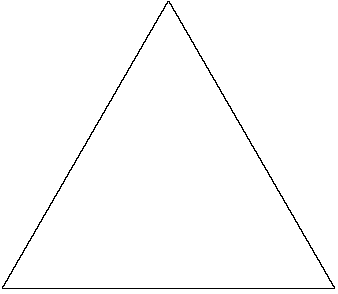
\includegraphics[scale=0.5]{./koch/triangle.png}
  \end{center}
\end{frame}

\begin{frame}{Step 2}
  \begin{center}
    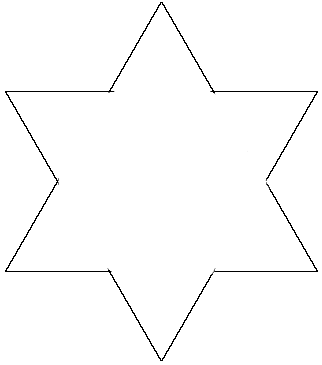
\includegraphics[scale=0.5]{./koch/step2.png}
  \end{center}
\end{frame}

\begin{frame}{Step 3}
  \begin{center}
    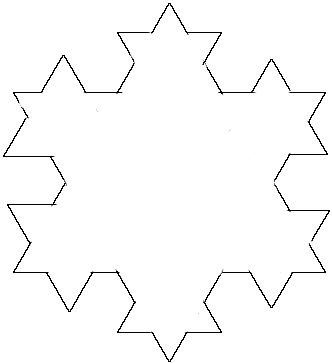
\includegraphics[scale=0.5]{./koch/step3.png}
  \end{center}
\end{frame}

\begin{frame}{A While Later...}
  \begin{center}
    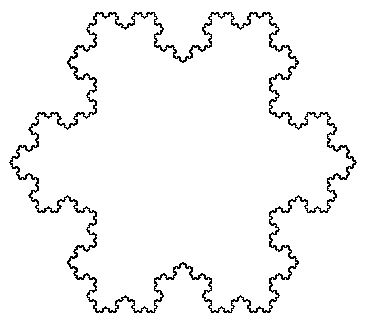
\includegraphics[scale=0.5]{./koch/koch-snowflake.png}\\
    \cite{Mathtricks}
  \end{center}
\end{frame}

\begin{frame}{Some Counting}
  At each step, we can see that the number of sides increases fourfold and the length of each side, $\eta$ decreases in length by a third.
  So, at the $n^{\text{th}}$ step we have side length $\eta = \eta(n) = d/3^n$ and the perimeter is given by $$L_{\eta} = \eta\cdot 4^n \cdot 3 = 3d\left(\frac{4}{3}\right)^n.$$
  
\end{frame}

\begin{frame}{Fantastic! Now What?}
  Using $\eta = d/3^n$ we can obtain 
  $$n = \frac{\log(d/\eta)}{\log(3)},$$
  which we use in conjuction with the formula for the perimeter to obtain
  \begin{align*}
    \begin{split}
      L_{\eta} &= 3de^{n[\log(4) - \log(3)]}\\
      &= 3de^{\log(d/\eta)(\log(4)/\log(3) - 1)}\\
      &= 3d\left(\frac{d}{\eta}\right)^{\alpha},
    \end{split}
  \end{align*}
  where $\alpha = \log(4)/\log(3) - 1 < 1.$
\end{frame}

\begin{frame}{}
  Recall the circle and $n$-gon example where we derived $L_{\eta} = d\Phi(\eta/d)$.
  We now have $$L_{\eta} = d\cdot 3\left(\frac{\eta}{d}\right)^{-\alpha},$$
  so we find that $\Phi(\eta/d) = 3(\eta/d)^{-\alpha}$.
  But now we note that unlike the circle and $n$-gon example, $L_{\eta}$ tends to infinity as $n$ tends to infinity.
\end{frame}

\begin{frame}{Tying Up Loose Ends}
  It turns out Richardson determined that the correct representation of the coastline is of the same type as the (von) Koch snowflake/triad.
  Indeed, if we let $\lambda = 3d^{1+\alpha}$ and $D = 1 + \alpha$, then $$L_{\eta} = d\cdot 3\left(\frac{\eta}{d}\right)^{-\alpha} = \lambda\eta^{1 - D},$$
  which has the same form as \eqref{1}.
\end{frame}

\begin{frame}{Some Cantor-esque Nonsense}
  We can now count the number of line segments 
  $$N_{\eta} = L_{\eta}/\eta = \lambda\eta^{-D}$$
  and construct squares on these segments, with a total area given by
  $$N_{\eta}\eta^2 = \lambda\eta^{2-D}.$$
  Remember that $\alpha < 1$ and thus $D = 1 + \alpha < 2$.
  Hence $2 - D > 1$ implies that the area tends to zero as $\eta$ tends to zero.
  It appears we've constructed something with infinite length and zero area...
\end{frame}

\begin{frame}{Fractal Dimension}
  Now if, instead of squares, we construct objects of dimension $D$, where $1 < D < 2$ holds, then we have
  $$N_{\eta}\eta^D = \lambda,$$ 
  which tends to a non-zero (remember $\lambda = 3d^{1+\alpha}$ does not depend on $\eta$) limit as $\eta$ tends to zero.
  
  This brings us to the following definition:
  \begin{defn}
    The constant $D$ is called the {\it fractal dimension} of the curve considered.
  \end{defn}
  
  It turns out that the coastlines of Britain and Australia have fractal dimensions $D \simeq 1.24$ and $D \simeq 1.13$, respectively.  
\end{frame}

\begin{frame}{Fractal Curve}
  Finally, we formally define a fractal curve:
  \begin{defn}
    A fractal curve is a continuous curve for which the fractal dimension is strictly larger than unity: 
    $$D > 1.$$
  \end{defn}
  
\end{frame}

\begin{frame}{Bibliography}
  \begin{thebibliography}{}
  \bibitem[Mathtricks, 2011]{Mathtricks}
    Mathtricks.org
    \newblock {\em koch-snowflake.jpg}
    \newblock http://mathtricks.org/wp-content/uploads/2010/01/koch-snowflake.png
    
  \bibitem[Wikipedia, 2011]{Wiki}
    Wikipedia.org
    \newblock {\em Britain-fractal-coastline-combined.jpg}
    \newblock http://mirror.math.ku.edu/tex-archive/macros/latex/contrib/beamer/doc/beameruserguide.pdf
  \end{thebibliography}
\end{frame}
\end{document}
